% Options for packages loaded elsewhere
\PassOptionsToPackage{unicode}{hyperref}
\PassOptionsToPackage{hyphens}{url}
\PassOptionsToPackage{dvipsnames,svgnames,x11names}{xcolor}
%
\documentclass[
  number]{elsarticle}

\usepackage{amsmath,amssymb}
\usepackage{iftex}
\ifPDFTeX
  \usepackage[T1]{fontenc}
  \usepackage[utf8]{inputenc}
  \usepackage{textcomp} % provide euro and other symbols
\else % if luatex or xetex
  \usepackage{unicode-math}
  \defaultfontfeatures{Scale=MatchLowercase}
  \defaultfontfeatures[\rmfamily]{Ligatures=TeX,Scale=1}
\fi
\usepackage{lmodern}
\ifPDFTeX\else  
    % xetex/luatex font selection
\fi
% Use upquote if available, for straight quotes in verbatim environments
\IfFileExists{upquote.sty}{\usepackage{upquote}}{}
\IfFileExists{microtype.sty}{% use microtype if available
  \usepackage[]{microtype}
  \UseMicrotypeSet[protrusion]{basicmath} % disable protrusion for tt fonts
}{}
\makeatletter
\@ifundefined{KOMAClassName}{% if non-KOMA class
  \IfFileExists{parskip.sty}{%
    \usepackage{parskip}
  }{% else
    \setlength{\parindent}{0pt}
    \setlength{\parskip}{6pt plus 2pt minus 1pt}}
}{% if KOMA class
  \KOMAoptions{parskip=half}}
\makeatother
\usepackage{xcolor}
\setlength{\emergencystretch}{3em} % prevent overfull lines
\setcounter{secnumdepth}{5}
% Make \paragraph and \subparagraph free-standing
\makeatletter
\ifx\paragraph\undefined\else
  \let\oldparagraph\paragraph
  \renewcommand{\paragraph}{
    \@ifstar
      \xxxParagraphStar
      \xxxParagraphNoStar
  }
  \newcommand{\xxxParagraphStar}[1]{\oldparagraph*{#1}\mbox{}}
  \newcommand{\xxxParagraphNoStar}[1]{\oldparagraph{#1}\mbox{}}
\fi
\ifx\subparagraph\undefined\else
  \let\oldsubparagraph\subparagraph
  \renewcommand{\subparagraph}{
    \@ifstar
      \xxxSubParagraphStar
      \xxxSubParagraphNoStar
  }
  \newcommand{\xxxSubParagraphStar}[1]{\oldsubparagraph*{#1}\mbox{}}
  \newcommand{\xxxSubParagraphNoStar}[1]{\oldsubparagraph{#1}\mbox{}}
\fi
\makeatother


\providecommand{\tightlist}{%
  \setlength{\itemsep}{0pt}\setlength{\parskip}{0pt}}\usepackage{longtable,booktabs,array}
\usepackage{calc} % for calculating minipage widths
% Correct order of tables after \paragraph or \subparagraph
\usepackage{etoolbox}
\makeatletter
\patchcmd\longtable{\par}{\if@noskipsec\mbox{}\fi\par}{}{}
\makeatother
% Allow footnotes in longtable head/foot
\IfFileExists{footnotehyper.sty}{\usepackage{footnotehyper}}{\usepackage{footnote}}
\makesavenoteenv{longtable}
\usepackage{graphicx}
\makeatletter
\def\maxwidth{\ifdim\Gin@nat@width>\linewidth\linewidth\else\Gin@nat@width\fi}
\def\maxheight{\ifdim\Gin@nat@height>\textheight\textheight\else\Gin@nat@height\fi}
\makeatother
% Scale images if necessary, so that they will not overflow the page
% margins by default, and it is still possible to overwrite the defaults
% using explicit options in \includegraphics[width, height, ...]{}
\setkeys{Gin}{width=\maxwidth,height=\maxheight,keepaspectratio}
% Set default figure placement to htbp
\makeatletter
\def\fps@figure{htbp}
\makeatother

\makeatletter
\@ifpackageloaded{caption}{}{\usepackage{caption}}
\AtBeginDocument{%
\ifdefined\contentsname
  \renewcommand*\contentsname{Table of contents}
\else
  \newcommand\contentsname{Table of contents}
\fi
\ifdefined\listfigurename
  \renewcommand*\listfigurename{List of Figures}
\else
  \newcommand\listfigurename{List of Figures}
\fi
\ifdefined\listtablename
  \renewcommand*\listtablename{List of Tables}
\else
  \newcommand\listtablename{List of Tables}
\fi
\ifdefined\figurename
  \renewcommand*\figurename{Figure}
\else
  \newcommand\figurename{Figure}
\fi
\ifdefined\tablename
  \renewcommand*\tablename{Table}
\else
  \newcommand\tablename{Table}
\fi
}
\@ifpackageloaded{float}{}{\usepackage{float}}
\floatstyle{ruled}
\@ifundefined{c@chapter}{\newfloat{codelisting}{h}{lop}}{\newfloat{codelisting}{h}{lop}[chapter]}
\floatname{codelisting}{Listing}
\newcommand*\listoflistings{\listof{codelisting}{List of Listings}}
\makeatother
\makeatletter
\makeatother
\makeatletter
\@ifpackageloaded{caption}{}{\usepackage{caption}}
\@ifpackageloaded{subcaption}{}{\usepackage{subcaption}}
\makeatother
\ifLuaTeX
  \usepackage{selnolig}  % disable illegal ligatures
\fi
\usepackage[]{natbib}
\bibliographystyle{plainnat}
\usepackage{bookmark}

\IfFileExists{xurl.sty}{\usepackage{xurl}}{} % add URL line breaks if available
\urlstyle{same} % disable monospaced font for URLs
\hypersetup{
  pdftitle={Scraps},
  pdfauthor={Ryan Lima},
  colorlinks=true,
  linkcolor={blue},
  filecolor={Maroon},
  citecolor={Blue},
  urlcolor={Blue},
  pdfcreator={LaTeX via pandoc}}

\setlength{\parindent}{6pt}
\begin{document}

\begin{frontmatter}
\title{Scraps}
\author[]{Ryan Lima%
%
}



\cortext[cor1]{Corresponding author}

        





\end{frontmatter}
    
The connection between forests and water supplies is well documented.
Around 65\% of surface water in the western states originates from
forested lands, which cover just 29\% of the land area
\citep{brown_source_2005}. The average annual precipitation in the Lower
Colorado River Basin is about 330 \(mm\), and only about 10 \(mm\) of
that precipitation becomes streamflow, while much of the rest is lost to
evapotranspiration \citep{zou_streamflow_2010}. Regional studies have
found that up to 90\% of annual precipitation in semi-arid forests is
lost evapotranspiration
\citep{dore_recovery_2012, ha_evapotranspiration_2015, yaseef_ecohydrology_2010, hibbert1979}.
Sublimation has been shown to remove 10 - 90\% of snowfall in the
Colorado River Basin, while the remaining snowmelt provides over 80\% of
streamflow to the Colorado River \citep{lundquist_sublimation_2024}.
Over half of streamflow from the Upper Colorado River basin comes from
groundwater sources primarily recharged by snowmelt \citep{miller2016}.
Therefore, small reductions in evaporative losses could have out-sized
impacts on available water supplies, particularly enhancing groundwater
recharge in terrains underlain by karst lithology
\citep{hibbert1979, wyatt2013}.

** Papers on how thinning works primarily in snow-dominated systems**

This research aims to develop criteria for areas suitable for thinning
to enhance groundwater recharge. It focuses primarily on regional
studies to determine suitability criteria, which are likely the best
predictor of hydrologic response to treatment
\citep{wyatt_estimating_2013}.

\section{Regional Hydrologic Responses to
Treatment}\label{regional-hydrologic-responses-to-treatment}

Several regional studies link forest treatment to changes in stand-level
ecohydrology, including increased tree growth in Ponderosa Pines greater
soil moisture and total ecosystem moisture leading to increased drought
resilience \citep{sankey_regionalscale_2021, sankey_thinning_2022},
increased snow retention \citep{broxton_subseasonal_2023, belmonte2021},
greater streamflow \citep{baker_effects_1986}, water table rise
\[Denver et al in Prep \]{[}\citep{smerdon_overview_2009}{]}\citep{schenk_impacts_2020}
and increased springflow
\citep{schenk_impacts_2020}\[Hart prarie and hoxworth in prep\].

\subsection{Water Yield/Runoff}\label{water-yieldrunoff}

Several regional studies link forest treatment to increased streamflow
\citep{dwivedi_how_2024, biederman_streamflow_2022, broxton_subseasonal_2023}.
However, there appears to be a threshold response, with water yield
increasing only in treated forests receiving over 500mm of annual
precipitation or in snow-dominated forests
\citep{biederman_streamflow_2022, carroll_evaluating_2016, adams_ecohydrological_2012, zou_streamflow_2010, hibbert1979}.

\subsection{Soil Moisture and Drought
Resilience}\label{soil-moisture-and-drought-resilience}

A synthesis of several treatment types across Northern Arizona,
including thinning at various levels and prescribed burning, found that
treated sites had significantly greater total ecosystem moisture, making
forests more resilient to
drought\citep{sankey_regionalscale_2021, sankey_thinning_2022}.
Treatments were shown to increase tree growth, improving resilience to
drought in Ponderosa Pine forests\citep{rodman2024}. Thinned Ponderosa
Pine forests have higher soil moisture for two to eight years
post-thinning, a result also found in semi-arid forests around the
Mediterranean
\citep{belmonte_soil_2022, del_campo_global_2022, odonnell_vegetation_2021, del_campo_effectiveness_2019}.

\subsection{Justification}\label{justification}

\begin{itemize}
\item
  regional studies are the best predictor of hydrologic response to
  thinning in Arizona forests \citep{wyatt_estimating_2013}
\item
  A snythesis of all 4FRI treatments found that thinned and burned
  forests have signifiantly greater total ecosystem moisture and are
  thus more resilient to drought and wildfire
  \citep{sankey_regionalscale_2021}
\item
  Thinned forests are better buffered against drought impacts in terms
  of both soil moisture and tree health \citep{sankey_thinning_2022}.
\item
  Soil moisture and ET may be affected by thinning for 3.6 - 8.6 years
  \citep{del_campo_global_2022}.
\item
  Prescribed burning or thinning can increase tree growth, improving
  resilience to drought in ponderosa pine forests \citep{rodman2024}.
\item
  Thinned forests (around Flagstaff) have higher soil moisture at 25 and
  50cm in the first two years post-thinning \citep{belmonte_soil_2022}.
\item
  Thinning in semi-arid forests around the Mediterranean increased
  antecedent soil moisture and below ground hydrologic processes and
  increased deep soil moisture by 50mm/year over the control
  \citep{del_campo_effectiveness_2019}.
\item
  a review of 35 studies published from 1971 to 2018 found that thinning
  was more effective than clear-cutting in terms of increasing
  groundwater recharge due to reduced sublimation and evaporation.
  Springs can effectively monitor groundwater recharge effects in arid
  lands \citep{schenk_impacts_2020}.
\item
  A review of studies on forest mgmt effects on groundwater resources
  found that a rise in the water table can generally be expected
  following forest thinning in all forested landscapes
  \citep{smerdon_overview_2009}.
\end{itemize}

\subsubsection{Snow retention}\label{snow-retention}

\begin{itemize}
\item
  The effects of forest thinning and subsequent snowmelt are highly
  variable, with responses depending on forest structure and local
  climate, where thinning in dense and taller vegetation generally
  increases snow retention, thinning in shorter, less dense forests may
  decrease retention \citep{lewis_prediction_2023}.
\item
  In semi-arid forested watersheds, thinning can influence streamflow
  variability by modifying snowpack accumulation and melt, particularly
  in wetter years where thinning can either reduce or increase snow
  retention based on site-specific
  conditions.\citep{broxton_subseasonal_2023}.
\item
  Thinning in semi-arid forested watersheds can significantly impact
  streamflow by altering snowmelt timing, with reduced forest cover
  tending to delay snowmelt at warmer sites while advancing melt at
  cooler, snowpack-persistent sites \citep{dwivedi_how_2024}.
\item
  Thinned forests around Flagstaff have greater snow persistence at
  25\%-35\% canopy cover \citep{belmonte_uav-based_2021}
\item
  Thinned forests in Northern Arizona have more snow and soil moisture
  \citep{odonnell_vegetation_2021}
\item
  Found that thinned and burned vs.~control forests had varying rates of
  snowmelt and snow persistence. Canopy cover is most predictive of snow
  persistence \citep{donager_integrating_2021}.
\end{itemize}

\subsubsection{Thresholds in literature}\label{thresholds-in-literature}

\begin{itemize}
\item
  A review of 94 catchment studies showed that significant changes in
  water yield are correlated to forest growth in forests that receive
  600-1200 mm of mean annual precipitation Bosch and Hewlett, 1982 The
  caveat being there were not many coniferous forests studies in that
  precipitation range \citep{bosch_review_1982}.
\item
  \citep{adams_ecohydrological_2012} hypothesized that where annual
  precipitation exceeds \textasciitilde500 mm or water yield is
  dominated by snowmelt, watershed will experience significantly
  decreased evapotranspiration and increased flows if canopy cover is
  reduced by over 20\%. However, their recent observations suggest that
  in dry forests, water yield may decrease. More research is needed.
  This paper was focused on tree-die off not thinning.
\item
  \citep{carroll_evaluating_2016} found a threshold hydrologic response
  when evaluating the thinning of a snow-dominated semi-arid
  Pinyon-Juniper community in the Great Basin. They found that a
  positive water yield in thinned plots was only observed when
  precipitation exceeded 400mm annually (wet years)
\item
  \citep{biederman_streamflow_2022} suggests that disturbance will
  positively impact streamflow for a minimum of several years following
  disturbance in areas where mean annual precipitation exceeds
  \textasciitilde500mm. ``Presumably because below 500 mm, most
  precipitation is evaporated regardless of forest condition (Hibbert,
  1979)\[\@\]
\item
  \citep{zhang_response_2001} evaluated 250 worldwide catchment studies
  and found that the differences in ET between forested and non-forested
  catchments diminish in areas with annual rainfall less than 500 mm
\end{itemize}

\subsection{thinning decreases ET in some
circumstances}\label{thinning-decreases-et-in-some-circumstances}

\begin{itemize}
\item
  Reductions of canopy cover can increase ET of existing trees, and
  solar radiation increases ET
  \href{Chen\%20et\%20al.,\%202005;\%20Bennett\%20et\%20al.,\%202018}{@biederman\_recent\_2015}
\item
  Decreases in post-disturbance ET may be offset by increased soil
  evaporation, increasing net ET (Reed et al., 2016)
\item
  \citep{goeking_forests_2020} reviewed the hydrologic response of
  stand-replacing and non-stand-replacing disturbances and found that
  post-disturbance streamflow may increase, not change, or even
  decrease. Non-stand replacing fires---because of increased evaporation
  from higher sub-canopy radiation and increased transpiration from
  rapid post-disturbance growth can reduce water availability in some
  cases.
\end{itemize}

\section{Data \& Methods}\label{sec-data-methods}

\subsection{Weighted Suitability
Workflow}\label{weighted-suitability-workflow}

\subsubsection{Define}\label{define}

\begin{quote}
``define the goal, supporting criteria, and evaluation metrics for the
weighted suitability model.''
\end{quote}

\textbf{Here we define the goal of this suitability map--to locate areas
on the Mogollon Rim Ranger District in the Coconino National Forest
where thinning may increase groundwater recharge based on modeling of
criteria found in the literature quantifying the impact of thinning on
water yield in Regional studies of Semi-arid forests.}

\subsubsection{Suitability Criteria}\label{suitability-criteria}

\paragraph{Aspect}\label{aspect}

Aspect has a large impact on solar radiation.

\begin{quote}
Closer to 0 or 360 is desired, low suitability scores for closeness
\end{quote}

\begin{figure}[H]

{\centering 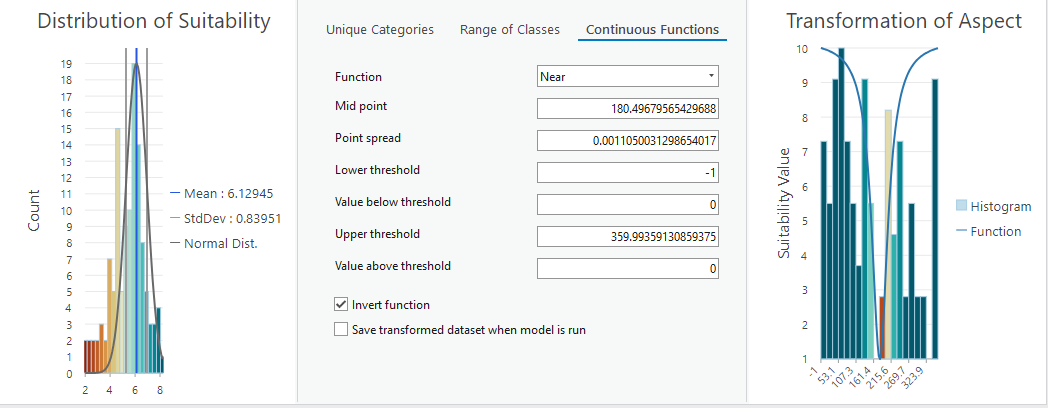
\includegraphics{images/Aspect_suitability.PNG}

}

\caption{Screenshot of Transfer function for Aspect Suitability}

\end{figure}%

\begin{center}\rule{0.5\linewidth}{0.5pt}\end{center}

\paragraph{Slope}\label{slope}

Higher slopes are less suitable because thinning is both more expensive,
and more precipitation will end up as runoff.

\begin{quote}
Lower slopes have higher suitability scores
\end{quote}

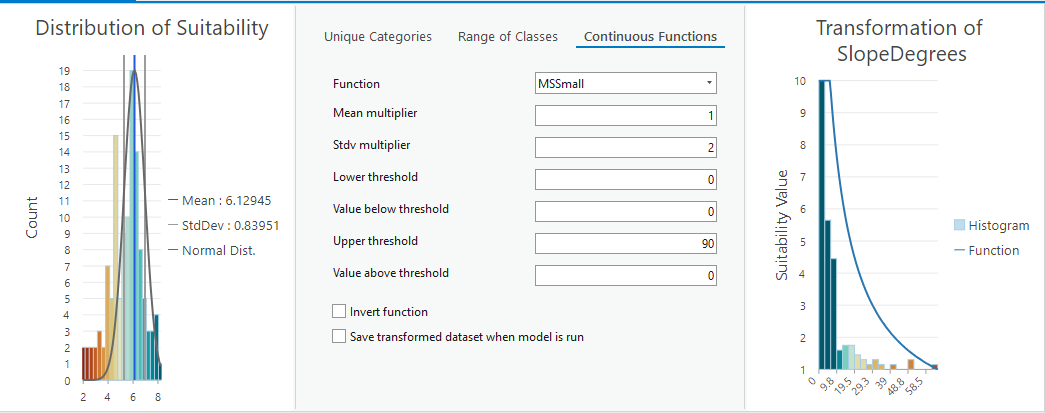
\includegraphics{images/Slope_suitability.PNG}

\begin{center}\rule{0.5\linewidth}{0.5pt}\end{center}

\paragraph{Elevation}\label{elevation}

Water yield in lower elevation watersheds will be less responsive to
changes in forest structure due to asynchrony between snowmelt and
transpiration \citep{biederman2022}

Winter precipitation mainly falls as snow at elevations above 1800m in
Arizona \citep{friederici2013}

\begin{center}\rule{0.5\linewidth}{0.5pt}\end{center}

\paragraph{Precipitation}\label{precipitation}

\begin{quote}
\textbf{Ideal:} Mean annual precipitation must be higher than 500mm 1990
- 2020

\textbf{Marginal:} (benefits only expected in wet years or during some
events) Max precipitation higher than 500mm but Mean annual
precipitation \textless{} 500mm

\textbf{Unsuitable:} Max annual precipitation \textless{} 500mm
\end{quote}

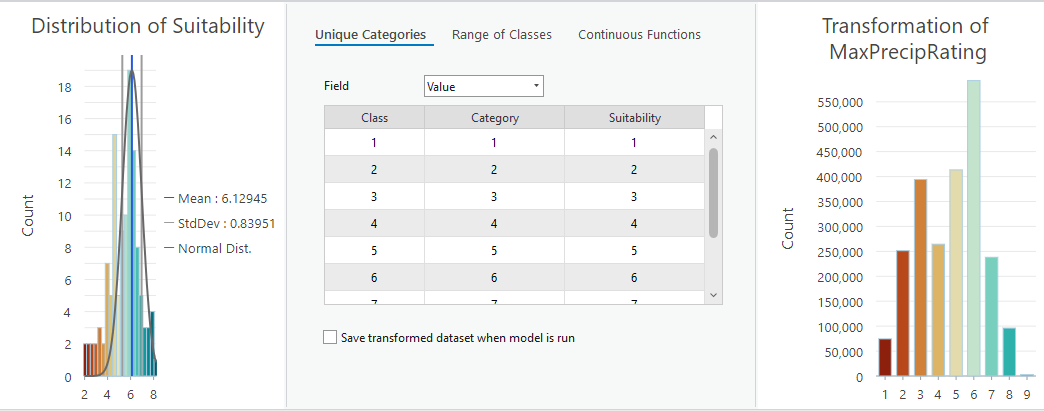
\includegraphics{images/Precipitation_suitability.PNG}

\begin{center}\rule{0.5\linewidth}{0.5pt}\end{center}

\paragraph{Vegetation Characteristics}\label{vegetation-characteristics}

Reconstructions of pre-settlement ponderosa pine forests have found a
range of canopy covers between 10 - 22\%, with a median of 16.7\% canopy
cover \citep{huffman2012}. However, remote sensing studies of snow
extent found that canopy covers of 24 - 35\% yield the ideal conditions
for maintaining snow cover \citep{sankey2015, belmonte2021a}. Which
means that restoring forests to pre-settlement canopy cover percentages
may not be the ideal canopy cover for maintaining snowpack, the dominant
source of groundwater recharge snow-dominant forest of Arizona.

Reductions in canopy cover of at least 20\% are likely required to see a
meaningful decrease in evapotranspiration \citep{adams2012}.

Because thinning is costly, and soil compaction from thinning operations
can adversely affect infiltration rates, we view a 20\% reduction as the
ideal canopy reduction to minimize cost and impact while meaningfully
reducing ET. A 20\% reduction in canopy cover with a starting canopy
cover of 20\%, yields a thinned canopy cover of 16\% canopy cover, the
median for pre-settlement forests, but probably on the low end for what
is ideal for maintaining snowcover, therefore we consider all areas with
forest cover below 21\% as unsuitable.

In order to maximize snow cover while reducing the canopy cover by 20\%,
we consider the ideal range of final canopy cover between 24\% - 35\%,
meaning the most suitable areas for thinning to maximize snow retention
would be forests with between 30\% and 44\%, with declining suitability
as the canopy cover deviates from that range. The function to convert
canopy cover then to suitability (1-10) is shown in equation
Equation~\ref{eq-cc-suitability}.

\begin{equation}\phantomsection\label{eq-cc-suitability}{y =\begin{cases} 10 \cdot \left(1 - \left(\frac{x - 37}{16 - 37}\right)^2\right),& \text{if } x < 37 \text{ and } x > 16, \\10 \cdot \left(1 - \left(\frac{x - 37}{80 - 37}\right)^2\right), & \text{if } x \geq 37 \text{ and } x < 80, \\0, & \text{if } x \leq 16 \text{ or } x \geq 80.\end{cases}}\end{equation}

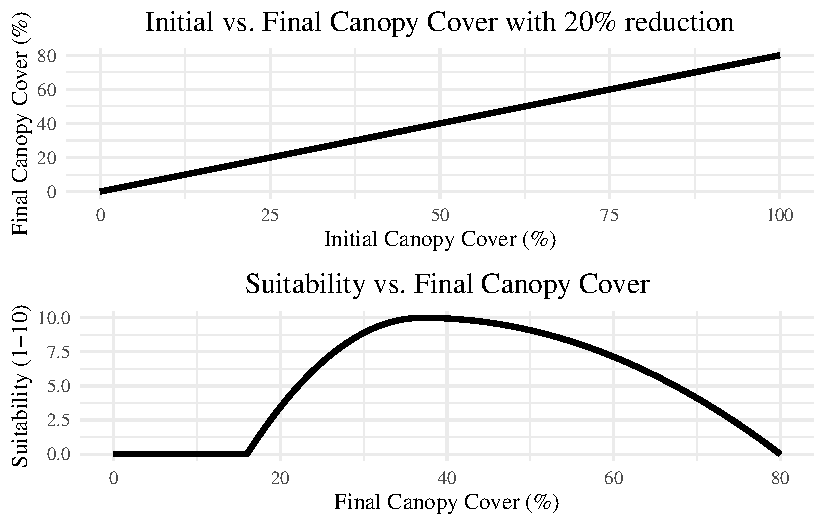
\includegraphics{scraps_files/figure-pdf/unnamed-chunk-1-1.pdf}

\begin{quote}
\textbf{Dataset: NLCD 2021 Total Canopy Cover (\% Cover)}
\end{quote}

\paragraph{Soil Hydrologic Conditions}\label{soil-hydrologic-conditions}

Soil types A,B,C,D are mapped for the USA, There are no A soil types in
the study area, so they were given the following suitability values

B = 10 out of 10 C = 8 out of 10 D = 3 out of 10

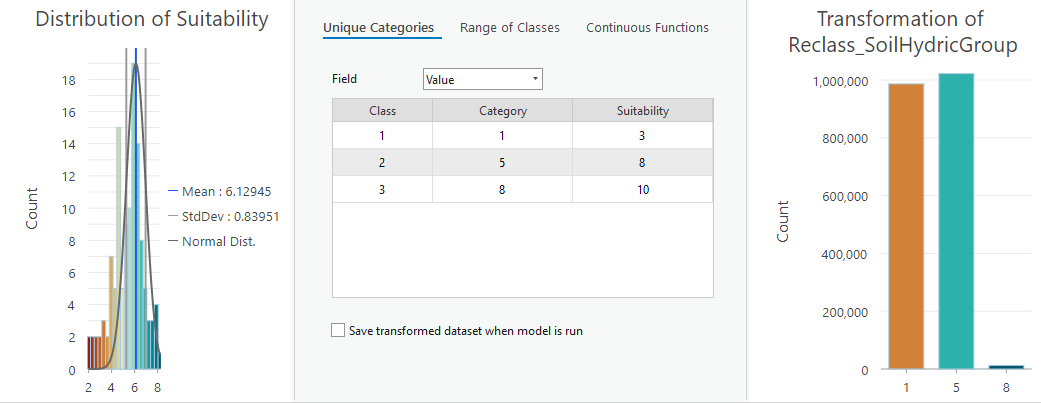
\includegraphics{images/SoilHydrologicGroup_suitability.PNG}

\section{Preliminary Results}\label{preliminary-results}

\subsection{Weighting}\label{weighting}

Tree Canopy Cover = 20\% Vegetation Condition Class = 20\% Slope = 20\%
Aspect = 20\% Max Precipitation = 15\% Soil Hydrologic Group = 5\%

\subsection{Overall Suitability}\label{overall-suitability}

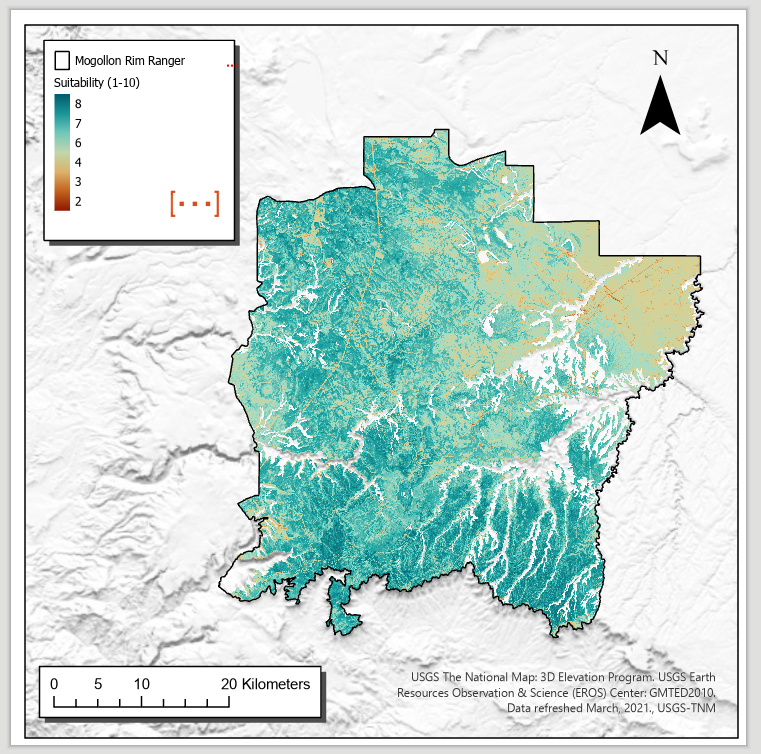
\includegraphics{images/PreliminarySuitabilityMap.PNG}

\begin{center}\rule{0.5\linewidth}{0.5pt}\end{center}



\end{document}
